\begin{frame}{Fitting assuming the 2-step reaction}
  \begin{tabular}{cc}
    \begin{minipage}{0.25\hsize}
      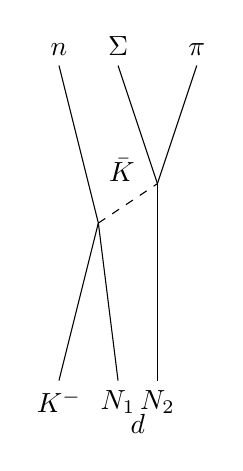
\begin{tikzpicture}
        \draw (-0.5, -2.0) node [below] {$K^-$} -- (0.0, 0.0) -- (-0.5, 2.0) node [above] {$n$};
        \draw (0.5,  -2.3) node [below] {$d$};
        \draw (0.25, -2.0) node [below] {$N_1$} -- (0.0, 0.0);
        \draw (0.75, -2.0) node [below] {$N_2$} -- (0.75, 0.5);

        \draw (0.3, 0.4) node [above] { $\bar{K}$ };
        \draw (0.0,  0.0) -- (0.75, 0.5) [dashed];
        
        \draw (0.75, 0.5) -- (1.25, 2.0)  node [above] {$\pi$};
        \draw (0.75, 0.5) -- (0.25, 2.0)  node [above] {$\Sigma$};
      \end{tikzpicture}
    \end{minipage}
    \begin{minipage}{0.75\hsize}
      \begin{eqnarray*}
        & & \frac{d\sigma}{dMd\Omega} = \int T_{K^-p \rightarrow \bar{K}N}\Phi_d(q_N2) G_0 T_{\bar{K}N \rightarrow \pi \Sigma} dq \\
        & & T_{\bar{K}N \rightarrow \pi \Sigma} = \frac{e^{i\delta}}{\sqrt{k_1}}
                                                  \frac{\sqrt{{\bf Im}A - \frac{1}{2}|A|^2{\bf Im}R k^2 }}{1 - iAk_2 + \frac{1}{2}ARk_2^2} \\
        & & T_{\bar{K}N \rightarrow \bar{K}N} = \frac{A}{1 - iA k_2 + \frac{1}{2}ARk_2^2} \\
        & & \Rightarrow (\mbox{Pole position}) : 1 - iA k_2 + \frac{1}{2}ARk_2^2 = 0                                          
      \end{eqnarray*}

    \end{minipage}
  \end{tabular}

  This fitting 2-complex, A \& R param and scaling factor.\\
  \hspace{5mm} $\Rightarrow$ 5 parameters
  
%%   \begin{thebibliography}{99}
%%     \scriptsize
%%   \bibitem{Gopal} \href{https://www.sciencedirect.com/science/article/abs/pii/0550321377900025}
%%     {G. P. Gopal et al., Nucl. Phys. B {\bf 119}, 362 (1977).}
%% %    {\\ "Partial-wave analyses of KN two-body reactions between 1480 and 2170 MeV"}
    
%%   \bibitem{d_fermi_theo} \href{https://journals.aps.org/prc/abstract/10.1103/PhysRevC.63.024001}
%%     {R. Machleidt, Phys. Rev. C{\bf 63}, 024001 (2001).}
    
%%   \bibitem{Miyagawa} \href{https://journals.aps.org/prc/abstract/10.1103/PhysRevC.85.065201}
%%     {K. Miyagawa and J. Haidenbauer, Phys. Rev. C {\bf 85}, 065201 (2012).}
%%   \end{thebibliography}
\end{frame}
  
